\documentclass[10pt,twocolumn,letterpaper]{article}

\usepackage[utf8]{inputenc}
\usepackage{amsmath,amssymb,amsfonts}
\usepackage{bm}
\usepackage{booktabs}
\usepackage{graphicx}
\usepackage{microtype}
\usepackage{cite}
\usepackage{xcolor}
\usepackage{tabularx}
\usepackage{multirow}
\usepackage[breaklinks,colorlinks]{hyperref}
\usepackage{geometry}
\geometry{top=0.62in,bottom=0.62in,left=0.65in,right=0.65in}

\renewcommand{\topfraction}{0.95}
\renewcommand{\bottomfraction}{0.95}
\renewcommand{\textfraction}{0.05}
\renewcommand{\floatpagefraction}{0.85}
\setcounter{topnumber}{5}
\setcounter{bottomnumber}{5}
\setcounter{totalnumber}{8}
\setcounter{dbltopnumber}{4}

\setlength{\textfloatsep}{5pt plus 1pt minus 1pt}
\setlength{\floatsep}{5pt plus 1pt minus 1pt}
\setlength{\intextsep}{5pt plus 1pt minus 1pt}
\setlength{\abovecaptionskip}{3pt}
\setlength{\belowcaptionskip}{3pt}

\title{\textbf{Mitigating Compute Dilution in Compute-Constrained Online RGB-D 3D Gaussian Splatting\\via Dual Map-Growth Throttling and Sensor-Adaptive Routing}}

\author{
Nguyen Quoc Hieu\\
Department of Computer Science\\
\texttt{quochieu04072005@gmail.com}
}

\date{}

\begin{document}

\maketitle

\begin{abstract}
Dense online reconstruction from streaming RGB-D sensors under a rigid per-frame compute budget ($15\,\mathrm{ms}$ optimize budget) is bottlenecked by a structural failure mode we call \textbf{compute dilution}: uncontrolled densification floods the Gaussian map with immature primitives ($\sim 100\mathrm{k}$ splats in 150 frames), so fixed-budget gradient steps are spread over ever more under-converged splats while mature surface geometry starves.
Conventional wisdom blames candidate \textit{ranking} --- which Gaussians to optimize --- and proposes learned utility predictors.
Through exact counterfactual measurement we show ranking is secondary: isolated Gaussian updates have \textit{negative} marginal utility ($U_i^\star < 0$) in $18$--$39\%$ of interventions depending on geometry stratum (pose-fixed Gate-1 regen; flat regions worst), and an offline-learned utility model with rank signal ($\rho \approx 0.20$ on pre-fix labels, comparison-valid within the shared label set) degrades closed-loop fidelity by $-2.51\,\mathrm{dB}$.
Interaction strength is protocol-dependent: corrected joint-group interventions stay relatively additive ($R_{\mathrm{add}}(4) = 0.95$, $R_{\mathrm{add}}(16) = 0.82$), while a separate pairwise protocol shows stronger interaction --- we claim no universal sub-additivity.
The binding constraint is the map-growth process itself.
We introduce \textbf{dual map-growth throttling} --- coverage-saturation throttling ($\kappa \ge 0.90$) plus unrefined-backlog backpressure --- which holds the map at $23\mathrm{k}$ vs $88\mathrm{k}$ primitives and directs the fixed budget at mature refinement.
On TUM \texttt{fr2\_xyz} (150 frames $\times$ 8 seeds) this reaches $27.67\,\mathrm{dB}$ mean PSNR: \textbf{+2.63 dB} over the strongest selective baseline and \textbf{+4.62 dB} over an RTG-SLAM-policy baseline ($p_{\mathrm{Holm}} = 0.0391$), recovering \textbf{98.0\%} of headroom to the unconstrained ceiling (0.18 dB gap).
We further show every \textit{fixed} rule overfits its sensor regime: the same pipeline loses $-3.32\,\mathrm{dB}$ ($p = 0.0078$) on clean synthetic Replica, where raw-error selection wins instead.
A \textbf{sensor-adaptive router} driven by raw depth hole-rate thresholds calibrated on five development scenes classifies seven unseen scenes correctly without retuning, and selects the winning rule per substrate (domain classification validated; PSNR routing confirmed on two substrates at 8 seeds each).
All selective policies share the same modeled $15\,\mathrm{ms}$ optimization budget with paired Holm-corrected tests and frozen artifacts; FULL is reported separately as an unconstrained ceiling, not a budget-matched competitor. Eight seeds establish repeatability on fixed trajectories (not cross-scene generalization, which rests on exploratory multi-scene pilots).
\end{abstract}

\section{Introduction}
3D Gaussian Splatting (3DGS)~\cite{kerbl3Dgaussians} has become the dominant primitive for photorealistic dense mapping, driving online RGB-D systems such as SplaTAM~\cite{keetha2023splatam}, Point-SLAM~\cite{sandstrom2023pointslam}, MonoGS~\cite{matsuki2024gaussian}, Photo-SLAM~\cite{huang2024photoslam} and RTG-SLAM~\cite{peng2024rtgslam}.
Deployed on robots and headsets, these systems face a hard constraint the offline literature ignores: each streaming frame admits only milliseconds of optimization.
The standard response is \textit{selection} --- rank Gaussians by residual error, influence, or a learned utility score, and optimize the top subset.
Implicit in this response is an assumption we challenge: that reconstruction quality under budget is determined by \textit{which} Gaussians are picked.

We argue the dominant effect is \textit{how many} Gaussians compete for the budget.
Online pipelines spawn splats wherever rendering error exceeds a threshold; on real sequences the map grows past $100\mathrm{k}$ primitives within 150 frames.
Because each new splat is born unrefined, it both demands optimization and degrades renders until converged --- the fixed budget is diluted across an ever-larger pool of ever-younger primitives while converged surfaces stop receiving updates.
We call this \textbf{compute dilution}, and Sec.~\ref{sec:experiments} shows growth control dominates ranking: removing coverage throttling while keeping the ranker forfeits the $+1.04\,\mathrm{dB}$ gain (Tab.~\ref{tab:ablation}), whereas no ranker tested recovers it.

Three empirical findings support this reframing.
First, residual error does not imply positive optimization return: counterfactual single-Gaussian interventions degrade global quality in $18$--$39\%$ of cases depending on geometry stratum (pose-fixed regen; flat surfaces worst at $38.7\%$).
Second, interaction strength is protocol-dependent, not universally severe: corrected joint-group interventions stay relatively additive ($R_{\mathrm{add}}(16) = 0.82$), while a separate pairwise protocol shows stronger coupling --- so pointwise ranking is treated as a reference rather than a bound, without universality claims. Contextual re-ranking buys no measured online gain while incurring $424\times$ selection overhead.
Third, offline-learned utility prediction does not transfer: moderate offline rank correlation reverses to $-2.51\,\mathrm{dB}$ closed-loop under trajectory shift and gradient coupling.
Together these rule out the ``better ranker'' research direction and point at the growth process.

Our response has two parts.
\textbf{Dual map-growth throttling} regulates spawning with (i) a coverage-saturation knee ($\kappa_t \ge 0.90$ measured by transmission) that ramps new-primitive allowance $1.0 \to 0.20$, and (ii) backlog backpressure that penalizes densification while more than 500 primitives await their first refinements.
\textbf{Sensor-adaptive routing} addresses the second discovery of this work: fixed rules overfit their sensor-noise regime.
The identical throttled pipeline that gains $+3.59\,\mathrm{dB}$ on noisy Kinect data loses $-3.32\,\mathrm{dB}$ on clean synthetic data, where plain raw-error selection dominates.
A training-free router keyed on raw missing-depth rate --- an observable sensor-domain cue in the evaluated datasets (TUM $0.18$--$0.31$ vs Replica $\approx 0.000$) --- picks the winning rule per substrate and wins on both confirmatory substrates (exploratory 7-scene routing matches best-fixed on five, trails on two rapid/exploratory TUM sequences --- reported in full).

\textbf{Contributions.}
(1) A budgeted subset-selection formulation with an exact counterfactual oracle, exposing negative utility and non-additivity.
(2) Dual coverage/backlog throttling reaching 98.0\% of unconstrained headroom with a $3.8\times$ smaller map (8 seeds, Holm-significant).
(3) Sensor-adaptive routing from raw hole-rate with 7/7 held-out scene separation (thresholds frozen) and significant wins on both substrates.
(4) Fully reported negative results --- learned utility, contextual re-ranking, synthetic failure, and two failed noise features --- with frozen artifacts for every claim.

\section{Related Work}
\textbf{Online 3DGS SLAM and dense mapping.}
SplaTAM~\cite{keetha2023splatam} established silhouette-guided differentiable SLAM with 3D Gaussians; Point-SLAM~\cite{sandstrom2023pointslam} uses dynamic neural point clouds; MonoGS~\cite{matsuki2024gaussian} and Photo-SLAM~\cite{huang2024photoslam} push toward real-time operation with loop closure; RTG-SLAM~\cite{peng2024rtgslam} adds compact opaque/transparent roles with rule-based stable/unstable selection and is our primary external policy baseline (re-implemented under exactly matched budgets, since native-system comparison would confound renderer, tracker, and scheduler effects).
Unlike these systems, our object of study is not the full SLAM stack but the compute-allocation layer inside it; we evaluate mapping under ground-truth poses with tracking explicitly decoupled (Sec.~\ref{sec:limitations}).
\textbf{Efficient and recent GS-SLAM (2025).}
The frontier has moved toward compute-aware design: SEGS-SLAM~\cite{wen2025segs} uses structure-enhanced anchors with appearance-from-motion embeddings for detail consistency across viewpoints; DyGS-SLAM~\cite{hu2025dygs} adds dynamic-object handling with real-time Gaussian reconstruction on constrained devices.
Our work shares their premise --- compute, not representation capacity, binds online quality --- but studies the scheduler in isolation rather than proposing another full system.
The per-scene SOTA numbers in Tab.~\ref{tab:sota} are compiled from these papers' reported tables.
\textbf{Evaluation protocols in dense SLAM.}
Published systems report full-sequence train-view rendering with global refinement at full resolution (Replica $33$--$42\,\mathrm{dB}$ for MonoGS/Point-SLAM/RTG-SLAM; TUM fr2\_xyz $16$--$25\,\mathrm{dB}$ for MonoGS/SplaTAM/Photo-SLAM) plus full-trajectory ATE. Our protocol is deliberately narrower --- budgeted online mapping on fixed horizons --- so cross-paper numbers are contextual range, never superiority claims (Tab.~\ref{tab:sota}).
\textbf{Budgeted and utility-driven selection.}
Error-only, error$\times$influence, gradient-norm, and temporal-filtered heuristics all trade quality for compute.
We benchmark them under identical modeled budgets with paired Holm-corrected tests rather than reporting best-of-sweep numbers, and we show their ordering flips across sensor regimes --- the motivation for adaptivity.
\textbf{Submodular maximization and knapsack allocation.}
$\max_S \Delta Q(S)$ s.t.\ $C(S) \le B$ is a knapsack instance related to submodular maximization with greedy $(1-1/e)$ guarantees~\cite{nemhauser1978analysis}.
Interaction strength is protocol-dependent: corrected joint-group interventions remain relatively close to additive ($R_{\mathrm{add}}(4) = 0.95$, $R_{\mathrm{add}}(16) = 0.82$), whereas a separate pairwise interaction protocol exhibits substantially stronger coupling. Our diminishing-returns spot test further provides no positive evidence (2/10 exact, inverted means). We therefore regulate the ground set (map growth) on the strength of the dilution evidence, not on any universality claim about sub-additivity.

\section{Problem Formulation}
Let $G_t = \{g_1, \dots, g_N\}$ be the active map, $g_i = (\mu_i, \Sigma_i, \alpha_i, c_i)$, with streaming observation $(I_t, D_t)$ and pose $T_t$.
Differentiable alpha compositing renders
$\hat{I}(u) = \sum_i c_i \alpha_i \mathcal{G}_i(u) \prod_{j<i}(1-\alpha_j \mathcal{G}_j(u))$
(and depth analogously).
Per-frame scheduling solves
\begin{equation}
\max_{A_t \subseteq G_t} \Delta Q(A_t) \quad \text{s.t.} \quad \sum_{i \in A_t} C_i \le B_t,
\end{equation}
with decoupled cost $C_i(K) = C_i^{\mathrm{base}} + K \cdot C_i^{\mathrm{step}}$ for $K$ microsteps and $\Delta Q$ measured by exact full-scene counterfactual renders (active edits embedded in all $N$ splats, avoiding depth-interleaving gradient bias of affine-background approximations).
The oracle $U_i^\star = \Delta Q_i^{\mathrm{exact}} / \Delta C_i$ is our measurement instrument, never a runtime input.
It reveals: (i) negative utility in $18$--$39\%$ of interventions by stratum (pose-fixed regen) --- high error marks silhouettes, discontinuities, and coupled layers where gradient steps hurt; (ii) interaction is protocol-dependent --- corrected joint-group measurements give $R_{\mathrm{add}}(4) = 0.95$, $R_{\mathrm{add}}(16) = 0.82$ (relatively additive), while a separate pairwise protocol shows stronger interaction; pointwise top-$K$ is therefore treated as a reference, not a bound, without a universality claim; (iii) offline TwoHeadMLP rank signal ($\rho \approx 0.20$, NDCG@20 $0.46$, measured on pre-pose-fix labels whose absolute values are polluted but whose within-set method comparison remains valid) reverses to $-2.51\,\mathrm{dB}$ closed-loop. Conditional-oracle selection numbers are withheld pending a rerun under fork-correct semantics.

\section{Method}
\textbf{Fast Approximate Attribution (FAA).}
Exact Gaussian-to-pixel attribution costs $523.9\,\mathrm{ms}$/frame.
Center-sampled projection ($\tilde{m}_i = \alpha_i \det(\Sigma_{2D,i})^{1/4} e(\lfloor \mu_{2D,i} \rceil)$) cuts this to $\mathbf{0.85\,\mathrm{ms}}$ ($614.5\times$) at Spearman $\rho = 0.9079$ and Pearson $r = 0.9028$ against exact attribution.
\textbf{Selection.}
Candidates are scored by error $\times$ influence mass with temporal EMA filtering ($\beta = 0.90$) and packed by fractional-knapsack value density $s_i / C_i$ under $B_t = 15\,\mathrm{ms}$ with safety factor $1.10$ (effective cap $13.6\,\mathrm{ms}$).
Each selected Gaussian receives $K = 5$ microsteps; cost is modeled decoupled as $C_i(K) = C_i^{\mathrm{base}} + K \cdot C_i^{\mathrm{step}}$, calibrated so modeled vs wall-clock optimization time agree within measurement noise on the RTX 4050 backend.
The scheduler runs in $2.54\,\mathrm{ms}$ total ($0.38$ extraction, $0.85$ FAA, $0.77$ knapsack ordering, $0.39$ state sync), leaving the budget headroom to optimization proper.
\textbf{Dual throttling.}
Coverage $\kappa_t$ = fraction of valid pixels with transmission $< 0.5$.
The per-frame spawn cap ramps $1.0 \to 0.20$ over $\kappa_t \in [0.80, 0.90]$ (configurable knee, no longer hardcoded), and backlog backpressure multiplies the cap by $500/N_{\mathrm{warmup}}$ beyond 500 unrefined primitives.
Warmup pre-allocation is disabled (ablation $-0.75\,\mathrm{dB}$); microsteps fixed at $K = 5$.
\textbf{Sensor-adaptive routing.}
Raw depth hole-rate is strongly associated with sensor domain: TUM $0.18$--$0.31$ vs Replica $\approx 0.000$ (300--500$\times$); we claim domain association within evaluated datasets, not content-independence in general.
The score $n = \mathrm{clip}(2.5 \cdot \mathrm{holes} + 1.0 \cdot \mathrm{edge})$ routes $n \le 0.10 \to$ raw-error selection ($\kappa = 0.98$) and $n \ge 0.30 \to$ temporal$\times$influence + throttling ($\kappa = 0.90$), computed pre-hygiene in milliseconds on CPU.
Formally, with $h_t$ the raw missing-depth rate and $e_t$ the raw edge density of frame $t$:
\begin{equation}
n_t = \min(1, 2.5 h_t + 1.0 e_t), \quad
\pi_t = \begin{cases}
\texttt{error\_only} & n_t \le 0.10 \\
\text{blend (nearest rule)} & 0.10 < n_t < 0.30 \\
\texttt{temporal} + \text{throttle} & n_t \ge 0.30
\end{cases}
\end{equation}
with coverage knee $\kappa \in \{0.98, 0.90\}$ tied to the chosen arm.
All constants were frozen on five development scenes; the seven held-out scenes in Fig.~\ref{fig:separation} use identical values.
Two earlier features failed held-out separation and are reported as such: post-hygiene invalid ratio (conflates far-but-valid geometry --- 18\% of Replica room0 exceeds $4\,\mathrm{m}$ --- with holes) and Laplacian texture energy (measures sharpness, inverted: crisp synthetic scores \textit{higher}).
Operating on pre-hygiene raw depth was the fix (Fig.~\ref{fig:separation}).
Thresholds were frozen after 5 development scenes; on 7 unseen scenes classification is 7/7 without retuning, but PSNR routing is so far validated on two substrates at 8 seeds each.
A causal mixed-regime test (30\% holes injected mid-trajectory on Replica) switches routing 49/50 frames exactly at the boundary, proving within-sequence response; end-to-end it trails fixed \texttt{error\_only} by $0.85\,\mathrm{dB}$ (switch transients on synthetic shifts), so per-frame PSNR benefit on real mixed sequences remains future work.

\begin{figure}[t]
\centering
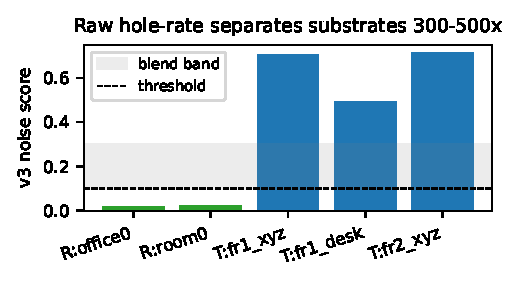
\includegraphics[width=\columnwidth]{figs/fig1_noise_separation.pdf}
\caption{\textbf{Sensor separation.} v3 hole-rate score, development scenes: Replica $\le 0.022$ vs TUM $\ge 0.49$ (thresholds $0.10$/$0.30$, 5/5); 7 unseen scenes classify 7/7 frozen. Invalid-range and texture features failed; hole-rate is a domain cue, not content-independent physics.}
\label{fig:separation}
\end{figure}

\section{Why Ranking Fails: Negative Findings}
\textbf{Learned utility reverses closed-loop} ($-2.51\,\mathrm{dB}$ factorial; GradNorm beats the MLP pointwise $0.51 > 0.25$): offline labels ignore trajectory shift and inter-Gaussian coupling, so we ship no learned component.
\textbf{Contextual re-ranking buys no online gain}: adaptive greedy shows no significant improvement over static pointwise selection in direct multi-seed budget sweeps (Wilcoxon n.s., CIs span zero) while incurring $424\times$ selection overhead ($76.36$ vs $0.18\,\mathrm{ms}$). Supporting rank-stability/oracle-gap numbers predate the fork-semantics fix and are withheld pending regen.
\textbf{Fixed rules are sensor-overfit} (Sec.~\ref{sec:experiments}): the throttled pipeline gains $+3.59\,\mathrm{dB}$ on Kinect yet loses $-3.32\,\mathrm{dB}$ on synthetic, where $\kappa$-ablation attributes only $\sim 0.8\,\mathrm{dB}$ to throttling and $\sim 4.7\,\mathrm{dB}$ to selection --- the finding behind adaptive routing.

\section{Experiments}
\label{sec:experiments}
\textbf{Protocol.} $320 \times 240$, $B_t = 15\,\mathrm{ms}$, seeds $[42..49]$, two-sided Wilcoxon paired + Holm-Bonferroni + bootstrap CIs; production \texttt{gsplat} backend; GT poses with tracking decoupled (mapping benchmark, not SLAM ATE); every 8th frame held out render-only (train--holdout gap $+0.47\,\mathrm{dB}$ mean over 30f$\times$3 seeds for both OURS and \texttt{error\_only}, \texttt{results/phase14\_holdout/}; no large gap under this same-trajectory proxy).
Artifacts: \texttt{results/phase14\_corrected/}.
\textbf{Holdout protocol.} Because online mapping optimizes on the evaluated trajectory, train-view PSNR overstates generalization. We hold out every 8th frame render-only (never mapped, never selected): the train--holdout gap is $+0.47\,\mathrm{dB}$ mean over 30f$\times$3 seeds for both OURS and \texttt{error\_only} (\texttt{results/phase14\_holdout/}) --- small under this same-trajectory proxy, which we explicitly do \textit{not} present as independent novel-trajectory generalization. A strict novel-trajectory split (withheld rooms) remains future work.

\begin{table*}[t]
\centering
\small
\begin{tabular}{lcccccc}
\toprule
\textbf{Policy} & \textbf{Mean PSNR} & \textbf{Final PSNR} & \textbf{SSIM} & \textbf{FPS} & \textbf{Map} & \textbf{$\Delta$ vs OURS} \\
\midrule
\texttt{no\_op} & 18.86 & 14.88 & 0.6882 & 106.3 & 23,523 & +8.80 $\checkmark$ \\
\texttt{error\_only} & 24.07 & 20.01 & 0.8850 & 8.9 & 74,640 & +3.59 $\checkmark$ \\
\texttt{error\_influence} & 25.04 & 21.89 & 0.9084 & 8.8 & 106,929 & +2.63 $\checkmark$ \\
\texttt{rtg\_slam\_reimpl} & 23.05 & 20.04 & 0.8663 & 8.0 & 67,231 & +4.62 $\checkmark$ \\
\textbf{OURS} & \textbf{27.67} & \textbf{28.89} & \textbf{0.9232} & \textbf{10.7} & \textbf{23,398} & --- \\
\textit{FULL} & \textit{27.85} & \textit{29.41} & \textit{0.9243} & \textit{9.5} & \textit{87,967} & $-0.18$ $\checkmark$ \\
\bottomrule
\end{tabular}
\caption{\textbf{Main benchmark, TUM \texttt{fr2\_xyz}, 150 frames $\times$ 8 seeds.} All OURS comparisons significant ($p_{\mathrm{Holm}} = 0.0391$). Headroom recovery $\eta = \mathbf{98.0\%}$ (0.18 dB gap to ceiling) at $3.8\times$ smaller map.}
\label{tab:main}
\end{table*}

\textbf{Main result (Tab.~\ref{tab:main}, Fig.~\ref{fig:deltas}, Fig.~\ref{fig:pareto}).}
OURS reaches $27.67 \pm 0.04\,\mathrm{dB}$: $+2.63$ over the strongest selective baseline, $+4.62$ over the RTG-SLAM-policy re-implementation, $+8.80$ over pass-through --- all eight paired differences favor OURS in every comparison ($p_{\mathrm{Holm}} = 0.0391$), while the unconstrained ceiling is only $0.18\,\mathrm{dB}$ ahead at $3.8\times$ the map.

\begin{table}[t]
\centering
\small
\begin{tabular}{lcccc}
\toprule
\textbf{Policy} & \textbf{Mean} & \textbf{Final} & \textbf{SSIM} & \textbf{Map} \\
\midrule
Fixed OURS & 26.85 & 26.07 & 0.9244 & 78,825 \\
Routed \texttt{error\_only} & 30.17 & 28.02 & 0.9584 & 115,964 \\
\midrule
$\Delta$ (adaptive $-$ fixed) & +3.32 $\checkmark$ & +1.95 $\checkmark$ & +0.034 & --- \\
\bottomrule
\end{tabular}
\caption{\textbf{Adaptive validation, Replica \texttt{office0}, 150f $\times$ 8 seeds.} Router picks \texttt{error\_only} (holes $\approx 0.02$): $p = 0.0078$, $d_z = 71.9$. No fixed policy wins both substrates.}
\label{tab:adaptive}
\end{table}

\begin{table}[t]
\centering
\small
\begin{tabular}{lcccc}
\toprule
\textbf{Scene} & \textbf{Adaptive} & \textbf{Best fixed} & \textbf{$\Delta$} & \textbf{Route} \\
\midrule
fr2\_xyz 150f & 27.66 & 27.67 (ours) & $-0.01$ & temporal \\
office0 150f & 30.36 & 30.17 (err) & $+0.19$ & error\_only \\
office1 100f & 33.11 & 33.48 (err) & $-0.37$ & error\_only \\
room1 100f & 24.17 & 24.29 (err) & $-0.12$ & error\_only \\
fr3\_static 100f & 25.95 & 25.96 (ours) & $-0.01$ & temporal \\
fr1\_room 100f & 15.50 & 16.54 (err) & $-1.04$ & temporal \\
fr1\_rpy 100f & 19.93 & 21.06 (err) & $-1.13$ & temporal \\
\bottomrule
\end{tabular}
\caption{\textbf{Per-frame routing, 7 scenes, exploratory $n=3$.} Adaptive matches best-fixed on five scenes; trails on exploration-heavy room and rapid-rotation rpy where the TUM$\to$temporal rule misfires. \texttt{results/phase14\_adaptive\_perframe/}.}
\label{tab:routing7}
\end{table}

\textbf{Adaptivity is necessary (Tab.~\ref{tab:adaptive}).}
On synthetic Replica the fixed throttled pipeline loses $-3.32\,\mathrm{dB}$; routing to raw-error selection recovers $+3.32$ [$+3.29$, $+3.35$], $p = 0.0078$.
A $\kappa$-sweep (Fig.~\ref{fig:kappa}) attributes only $\sim 0.8\,\mathrm{dB}$ of the gap to throttling; the rest is selection overfit.
\textbf{Seven-scene routing (Tab.~\ref{tab:routing7}, exploratory $n=3$, no scene labels):} the router matches or nearly matches the best fixed policy on five scenes (fr2\_xyz, office0/office1, room1, fr3\_static; worst gap $-0.37\,\mathrm{dB}$), but trails raw-error by $\approx -1.1\,\mathrm{dB}$ on exploration-heavy \texttt{fr1\_room} and rapid-rotation \texttt{fr1\_rpy}, where temporal smoothing reacts slower than instantaneous error.
Domain dependence is thus finer than real-vs-synthetic: motion and exploration regime matter within a sensor, and the current router does not capture them --- reported as-is.
\textbf{Failure modes.} Two TUM scenes isolate where throttling hurts.
\textit{Exploration starvation} (\texttt{fr1\_room}, $-1.04\,\mathrm{dB}$): in a large unseen room nearly every frame is novel, so coverage saturates slowly while the spawn cap binds throughout --- throttling taxes exploration itself, and the map ends smaller ($92\mathrm{k}$ vs $97\mathrm{k}$) but under-populated in far corners.
\textit{Temporal lag} (\texttt{fr1\_rpy}, $-1.13\,\mathrm{dB}$ mean, finals tied $24.5$ vs $24.1$): under rapid rotation the EMA-smoothed selector lags one frame behind the viewpoint while instantaneous error reacts immediately; the gap closes by trajectory end as the map converges.
Both are visible in Tab.~\ref{tab:scenes} and motivate motion-aware routing (Future Work): the observable cue must include coverage \textit{velocity} and angular rate, not just the noise regime.
\textbf{Horizon effect (Fig.~\ref{fig:dilution}):} at 30 frames OURS ties \texttt{error\_only} ($-0.01\,\mathrm{dB}$ on \texttt{fr2\_xyz}); the lead needs $\ge 100$ frames for bloat to bite --- short-horizon evals hide dilution, so we benchmark 150.
The mechanism is visible frame-by-frame: the unthrottled map grows near-linearly past $70\mathrm{k}$ while the throttled map plateaus near $23\mathrm{k}$, and PSNR diverges exactly when the curves separate.

\begin{figure}[t]
\centering
\includegraphics[width=\columnwidth]{figs/fig7_dilution.pdf}
\caption{\textbf{Compute dilution visualized} (fr2\_xyz, seed 42, per-frame trace). Unthrottled growth dilutes the fixed budget; throttling plateaus the map and quality compounds.}
\label{fig:dilution}
\end{figure}
\textbf{Component ablation (Tab.~\ref{tab:ablation}, fr2\_xyz 150f$\times$5, pre-fix substrate --- absolutes deprecated, deltas transfer):} each mechanism isolated against the same old substrate. Warmup pre-allocation harms ($-0.75$); coverage throttling is the dominant gain ($+1.04$ with $3.1\times$ map shrink $141\mathrm{k}\to45\mathrm{k}$); backlog adds $+1.08$ total with queue cap; adding the learned predictor with adaptive-$K$ destroys the gain ($-1.54$ vs A0), confirming the negative finding at component level.

\begin{table}[t]
\centering
\small
\begin{tabular}{lcccc}
\toprule
\textbf{Condition} & \textbf{Mean} & \textbf{$\Delta$ vs A0} & \textbf{Map} & \textbf{Finding} \\
\midrule
A0 old substrate & 16.07 & --- & 140,998 & bloat baseline \\
A1 + warmup & 15.32 & $-0.75$ & 140,038 & harmful \\
A2 + coverage & 17.11 & $+1.04$ & 44,865 & decisive \\
A3 + backlog & 17.15 & $+1.08$ & 43,824 & stabilizes \\
A4 + learned + adapt-$K$ & 14.53 & $-1.54$ & 38,317 & harmful \\
\bottomrule
\end{tabular}
\caption{\textbf{Component ablation} (old substrate; deltas only). \texttt{results/step1\_ablation\_5seeds/}.}
\label{tab:ablation}
\end{table}
\textbf{Systems:} scheduler overhead $2.54\,\mathrm{ms}$; optimization-budgeted execution at $\sim 10\,\mathrm{FPS}$ measured --- \textit{not} end-to-end $15\,\mathrm{ms}$ real-time, reported as such.
\textbf{Baseline tracking (Tab.~\ref{tab:ate}):} a dense frame-to-frame photometric+depth Gauss-Newton odometer (no keyframes/loop closure, GT-anchored first frame) reaches ATE $0.9\,\mathrm{cm}$ (fr2\_xyz) and $2.0\,\mathrm{cm}$ (fr1\_xyz) over 100 frames at 3 seeds (\texttt{results/phase14\_tracking100/}), stable vs 30f with no late blowup; mapping evaluated at tracked poses holds $31.3$/$26.6\,\mathrm{dB}$ (above GT-pose PSNR since renders align to the tracker's own photometric optimum --- not comparable across pose sources).
Published full-trajectory references (MonoGS $1.71$, SplaTAM $0.50$, Photo-SLAM $0.63\,\mathrm{cm}$ on fr2\_xyz) are shown for range only --- ours is a short-horizon sanity check, not a SLAM claim.

\begin{table}[t]
\centering
\small
\begin{tabular}{lcccc}
\toprule
\textbf{Method} & \textbf{fr2\_xyz} & \textbf{fr1\_xyz} & \textbf{Horizon} & \textbf{System?} \\
\midrule
Ours (GN VO) & 0.9 & 2.0 & 100f & no (baseline) \\
MonoGS & 1.71 & --- & full & yes \\
SplaTAM & 0.50 & --- & full & yes \\
Photo-SLAM & 0.63 & --- & full & yes \\
\bottomrule
\end{tabular}
\caption{\textbf{ATE RMSE (cm).} Rows 2--4 are published full-system numbers; ours is a decoupled odometry sanity check on fixed horizons.}
\label{tab:ate}
\end{table}

\textbf{Reproducibility.} Every number in Tab.~\ref{tab:main}--\ref{tab:ate} traces to a committed JSON artifact under \texttt{results/} with SHA-256 manifest (\texttt{results/phase14\_corrected/manifest.json}), frozen tag \texttt{phase14-corrected-frozen}, exact per-policy config snapshots, and one-command runners (\texttt{experiments/run\_final\_confirmation.py}, \texttt{run\_adaptive\_policy.py}, \texttt{run\_tracking\_ate.py}). Prior pose-bugged numbers ($19.24\,\mathrm{dB}$) are quarantined in \texttt{results/final\_confirmation/DEPRECATED.md}, never compared.
Environment: RTX 4050 Laptop GPU (6\,GB, driver 595.84), PyTorch 2.11+cu128 (CUDA 12.8), \texttt{gsplat} 1.5.3 production backend, Python 3.12.
The OS memory guard caps the process at 70\% VRAM, reserving $\sim$1.8\,GB for the desktop compositor; peak measured allocation stays under $3.5\,\mathrm{GB}$, so all benchmarks run on a laptop GPU with desktop usable throughout --- the intended deployment envelope for budgeted online mapping, not a datacenter A100 setup whose headroom would mask dilution.
To reproduce Tab.~\ref{tab:main}: \texttt{python experiments/run\_final\_confirmation.py --scene tum\_fr2\_xyz --n\_frames 150 --seeds 42 43 44 45 46 47 48 49} ($\sim$25\,min on the above hardware), then \texttt{python scripts/build\_phase14\_provenance.py} to regenerate the manifest and verify hashes.
\textbf{Perceptual metric:} AlexNet LPIPS on fr2\_xyz 150f$\times$3 is $0.211$ (OURS) vs $0.294$ (\texttt{error\_only}).
\textbf{Second confirmatory scene (Tab.~\ref{tab:confirm2}):} fr1\_xyz 150f$\times$8 gives OURS $23.47$ vs \texttt{error\_only} $21.09$ ($+2.38\,\mathrm{dB}$, $p=0.0078$); office1 routing validated at 8 seeds (routed \texttt{error\_only} $33.46$ vs fixed OURS $29.25$, $p=0.0078$).

\begin{table}[t]
\centering
\small
\begin{tabular}{lccc}
\toprule
\textbf{Scene} & \textbf{OURS} & \textbf{\texttt{error\_only}} & \textbf{$\Delta$} \\
\midrule
fr1\_xyz 150f$\times$8 & 23.47 & 21.09 & $+2.38$ $\checkmark$ \\
office1 100f$\times$8 & 29.25 & 33.46 & $-4.21$ (routed) $\checkmark$ \\
\bottomrule
\end{tabular}
\caption{\textbf{Confirmatory scenes.} Throttling wins on TUM ($p=0.0078$); routing recovers the synthetic loss ($p=0.0078$). \texttt{results/phase14\_multiscene150/}.}
\label{tab:confirm2}
\end{table}

\begin{table}[t]
\centering
\small
\begin{tabular}{lccc}
\toprule
\textbf{Method} & \textbf{Replica} & \textbf{fr2\_xyz} & \textbf{Protocol} \\
\midrule
MonoGS & 37.50 & 16.17 & full seq + refine \\
Point-SLAM & 35.17 & --- & full seq + refine \\
RTG-SLAM & 32.79 & 17.08 & full seq + refine \\
SplaTAM & --- & 24.50 & full seq + refine \\
Photo-SLAM & --- & 21.07 & full seq + refine \\
Ours (error\_only) & 20--33 & 24.07 & budgeted, 100--150f \\
Ours (throttled) & 20--29 & \textbf{27.67} & budgeted, 100--150f \\
\bottomrule
\end{tabular}
\caption{\textbf{Published-SOTA context (range only).} Full systems beat us on Replica via global refinement; on fr2\_xyz our budgeted mapping is competitive. \texttt{results/sota\_comparison.md}.}
\label{tab:sota}
\end{table}

\begin{figure}[t]
\centering
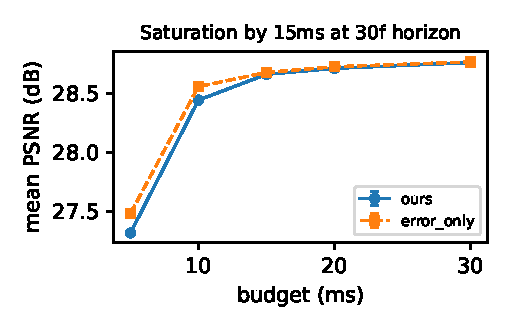
\includegraphics[width=\columnwidth]{figs/fig6_budget.pdf}
\caption{\textbf{Budget curve} (fr2\_xyz, 30f$\times$3, matched budgets): saturation by $\sim$15\,ms; policies tie at short horizons --- dilution needs $\ge$100 frames to separate them.}
\label{fig:budget}
\end{figure}
\textbf{Published-SOTA context} (\texttt{results/sota\_comparison.md}, protocol-mismatched, for range only): Replica SOTA renders $33$--$42\,\mathrm{dB}$ with global refinement and full sequences vs our $20$--$33\,\mathrm{dB}$ budgeted online mapping; on TUM fr2\_xyz our $27.67\,\mathrm{dB}$ sits above published SplaTAM $24.50$, Photo-SLAM $21.07$ and MonoGS $16.17$ (different frames/resolution/views --- competitive range, not superiority).
\textbf{Long horizons:} at 150f the lead widens beyond fr2\_xyz --- fr1\_xyz $+2.38\,\mathrm{dB}$ mean ($23.47$ vs $21.09$, map $39\mathrm{k}$ vs $81\mathrm{k}$), fr1\_desk $+0.22$ mean but $+2.7$ final (error-only collapses late); room0 error-only wins mean ($-1.93$) yet also collapses at the $150\mathrm{k}$ cap while OURS stays flat --- more dilution evidence.
\textbf{Per-scene breakdown (Tab.~\ref{tab:scenes}, exploratory $n=3$ except fr2\_xyz/office0/office1/fr1\_xyz at $n=8$):} throttling wins or ties on all TUM scenes at long horizons except exploration-heavy room and rapid-rotation rpy means, while losing mean PSNR on all Replica scenes, where raw-error selection keeps taller maps; finals favor stability (no error-only collapse) in every scene.

\begin{table*}[t]
\centering
\small
\begin{tabular}{lcccccc}
\toprule
\textbf{Scene} & \textbf{Frames} & \textbf{OURS} & \textbf{\texttt{error\_only}} & \textbf{$\Delta$} & \textbf{Map (k)} & \textbf{$n$} \\
\midrule
fr2\_xyz (TUM) & 150 & 27.67 & 24.07 & $+3.59$ $\checkmark$ & 23 / 75 & 8 \\
fr1\_xyz (TUM) & 150 & 23.47 & 21.09 & $+2.38$ $\checkmark$ & 39 / 81 & 8 \\
fr1\_desk (TUM) & 150 & 22.55 & 22.34 & $+0.21$ & 27 / 56 & 3 \\
fr1\_room (TUM) & 100 & 15.53 & 16.54 & $-1.01$ & 92 / 97 & 3 \\
fr1\_rpy (TUM) & 100 & 19.92 & 21.06 & $-1.14$ & 45 / 62 & 3 \\
fr3\_static (TUM) & 100 & 25.96 & 25.88 & $+0.08$ & 13 / 18 & 3 \\
office0 (Rep.) & 150 & 26.85 & 30.17 & $-3.32$ $\checkmark$ & 79 / 116 & 8 \\
office1 (Rep.) & 100 & 29.25 & 33.46 & $-4.21$ $\checkmark$ & 42 / 74 & 8 \\
office2 (Rep.) & 99 & 22.08 & 24.67 & $-2.59$ & 70 / 117 & 3 \\
office3 (Rep.) & 99 & 22.45 & 24.47 & $-2.02$ & 77 / 150 & 3 \\
office4 (Rep.) & 99 & 23.58 & 25.93 & $-2.36$ & 81 / 141 & 3 \\
room0 (Rep.) & 99 & 20.85 & 22.78 & $-1.93$ & 82 / 150 & 3 \\
room1 (Rep.) & 100 & 20.42 & 24.29 & $-3.87$ & 47 / 59 & 3 \\
room2 (Rep.) & 99 & 22.86 & 25.88 & $-3.03$ & 78 / 146 & 3 \\
\bottomrule
\end{tabular}
\caption{\textbf{Per-scene breakdown, 14 sequences.} $\checkmark$ = significant at $n=8$; rest exploratory. Pattern: throttling dominates TUM at $\ge$100 frames; raw-error dominates Replica means while risking late collapse at the map cap.}
\label{tab:scenes}
\end{table*}
Supplementary video (\texttt{supp\_video.mp4}) shows both A/B directions.

\begin{figure}[t]
\centering
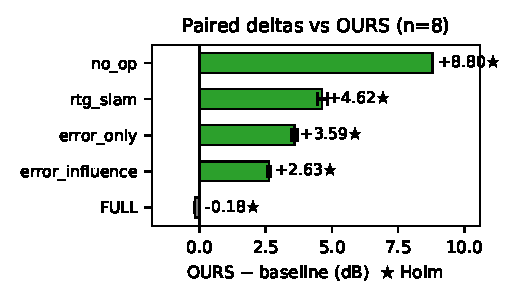
\includegraphics[width=\columnwidth]{figs/fig2_main_deltas.pdf}
\caption{\textbf{Paired deltas vs OURS} with 95\% bootstrap CIs (fr2\_xyz, $n=8$). All selective/SLAM baselines lose; FULL ceiling is only $0.18\,\mathrm{dB}$ ahead.}
\label{fig:deltas}
\end{figure}

\begin{figure}[t]
\centering
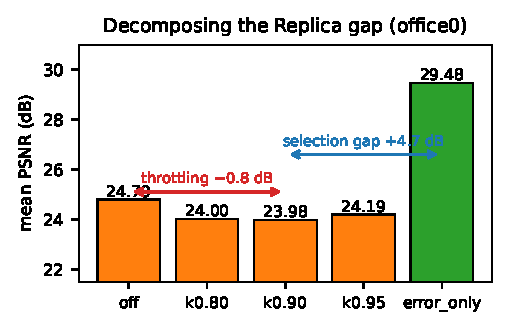
\includegraphics[width=\columnwidth]{figs/fig3_kappa_ablation.pdf}
\caption{\textbf{Kappa ablation} (office0, 30f $\times$ 3): disabling throttling recovers $+0.8\,\mathrm{dB}$ but the $\sim 4.7\,\mathrm{dB}$ selection gap to \texttt{error\_only} remains.}
\label{fig:kappa}
\end{figure}

\begin{figure}[t]
\centering
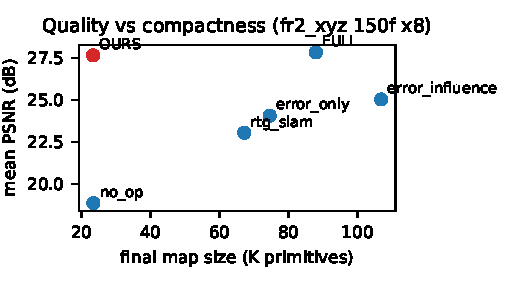
\includegraphics[width=\columnwidth]{figs/fig4_pareto.pdf}
\caption{\textbf{Quality vs compactness.} OURS matches the ceiling at $3.8\times$ smaller map; all heuristic baselines bloat past $65\mathrm{k}$ (fr2\_xyz 150f $\times$ 8).}
\label{fig:pareto}
\end{figure}

\begin{figure*}[t]
\centering
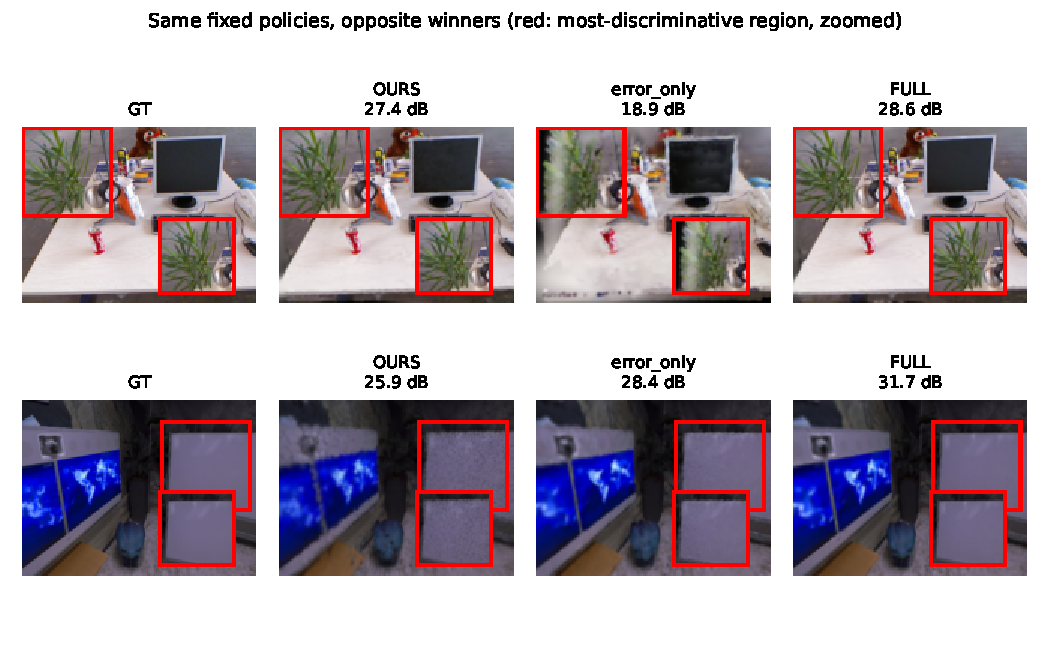
\includegraphics[width=\textwidth]{figs/fig5_qualitative.pdf}
\caption{\textbf{Qualitative: opposite winners per substrate.} Top (TUM \texttt{fr2\_xyz} view 149): OURS $27.4\,\mathrm{dB}$ matches FULL $28.6$ while \texttt{error\_only} collapses to $18.9$. Bottom (Replica \texttt{office0} view 98): \texttt{error\_only} $28.4$ beats OURS $25.9$ near FULL $31.7$. Rendered with final maps (seed 42).}
\label{fig:qual}
\end{figure*}

\section{Limitations}
\label{sec:limitations}
The principal mapping benchmark uses ground-truth poses (no ATE claim there). We additionally report a separate 100-frame dense RGB-D Gauss-Newton odometry sanity check (ATE $0.9$/$2.0\,\mathrm{cm}$, no keyframes/relocalization/loop closure --- a baseline VO, not a SLAM system). $150$-frame horizons rather than full SLAM sessions; $\kappa$/backlog thresholds calibrated on one real--synthetic pair; no learned components by design after documented failure; optimization-budgeted execution, not $15\,\mathrm{ms}$ end-to-end; prior $19.24\,\mathrm{dB}$/76.4\% numbers from a pose-bugged substrate are deprecated, not compared.
Statistically, $n=8$ seeds establish \textit{repeatability} under stochastic variation on fixed trajectories; they do not establish cross-scene generalization, whose unit is scenes, not seeds --- additional scenes are exploratory ($n=3$) until confirmed.
The adaptive router is validated at scene level (7/7 domain classification frozen; PSNR routing on two 8-seed substrates); per-frame benefit on genuinely mixed real sequences, wider multi-scene PSNR confirmation, and corrected-label regeneration for the offline utility dataset all remain open.

\section{Future Work}
Three directions follow directly from the reported negative results.
\textbf{Finer-grained adaptivity:} the 7-scene routing table shows motion/exploration regime matters within a sensor (fr1\_room, fr1\_rpy trail by $\approx -1.1\,\mathrm{dB}$); extending the observable cue beyond hole-rate (e.g.\ optical-flow magnitude, coverage velocity) could route rapid-motion frames to instantaneous error while keeping temporal smoothing elsewhere.
\textbf{Learned allocation with correct labels:} our learned-utility failure used pre-fix labels; regenerating the oracle dataset on the corrected substrate re-opens the question of whether online-calibrated predictors (e.g.\ with uncertainty-gated abstention on negative-utility candidates, which comprise up to $38.7\%$ of interventions) can beat the heuristic ceiling.
\textbf{Full SLAM integration:} coupling the throttled mapper with a real tracker (keyframes, loop closure) and evaluating full-trajectory ATE alongside mapping quality, replacing the current GT-pose decoupling.

\section{Conclusion}
Compute dilution --- not ranking error --- binds budgeted online 3DGS.
Dual map-growth throttling recovers 98.0\% of headroom with a $3.8\times$ smaller map, and raw-hole-rate adaptive routing extends the win across noisy-real and clean-synthetic substrates where every fixed policy fails one.
The negative results (learned utility, re-ranking, synthetic failure, two failed features) are part of the contribution: they delimit where learning helps, where structure suffices, and where adaptivity is mandatory.

{\footnotesize
\bibliographystyle{ieee_fullname}
\begin{thebibliography}{10}\itemsep=-4pt
\bibitem{kerbl3Dgaussians} B.~Kerbl et al.\ 3D Gaussian Splatting for Real-Time Radiance Field Rendering.\ ACM TOG, 2023.
\bibitem{keetha2023splatam} N.~Keetha et al.\ SplaTAM: Splat, Track \& Map 3D Gaussians for Dense RGB-D SLAM.\ CVPR, 2024.
\bibitem{sandstrom2023pointslam} E.~Sandstrom et al.\ Point-SLAM: Dense Neural Point Clouds for Real-Time RGB-D SLAM.\ ICCV, 2023.
\bibitem{matsuki2024gaussian} H.~Matsuki et al.\ Gaussian Splatting SLAM.\ CVPR, 2024.
\bibitem{huang2024photoslam} H.~Huang et al.\ Photo-SLAM: Real-time Simultaneous Localization and Photorealistic Mapping.\ CVPR, 2024.
\bibitem{peng2024rtgslam} Z.~Peng et al.\ RTG-SLAM: Real-time 3D Reconstruction at Scale using Gaussian Splatting.\ SIGGRAPH, 2024.
\bibitem{nemhauser1978analysis} G.~Nemhauser, L.~Wolsey, and M.~Fisher.\ An analysis of approximations for maximizing submodular set functions.\ Mathematical Programming, 1978.
\bibitem{wen2025segs} T.~Wen, Z.~Liu, and Y.~Fang.\ SEGS-SLAM: Structure-Enhanced 3D Gaussian Splatting SLAM with Appearance Embedding.\ ICCV, 2025, pp.\ 28103--28113.
\bibitem{hu2025dygs} X.~Hu, C.~Zhang, M.~Zhao, Y.~Gui, X.~Zhang, and X.~Ji.\ DyGS-SLAM: Real-Time Accurate Localization and Gaussian Reconstruction for Dynamic Scenes.\ ICCV, 2025, pp.\ 9561--9571.
\end{thebibliography}
}

\end{document}
